
\subsection{Contributing to \aspect}

\begin{enumerate}
\item make sure that you  have an account on GitHub (say, \verb"https://github.com/myusername") 
and carry out a proper setup on your local computer as follows:\\
\verb'$ git config --global user.name "firstname lastname" '\\
\verb'$ git config --global user.email your@email'

\item On github.com, fork the official \aspect repository to your repository:\\
go to \verb"https://github.com/geodynamics/aspect"
and click on the 'fork' button on the upper right corner of the screen.

\item On your machine, in a terminal, clone your repository with \\
\verb"$ git clone git@github.com:myusername/aspect.git". 
This is now your main\footnote{previously 'master', although this term should not be used anymore} branch.

\item 
Follow the instructions at \url{https://docs.github.com/en/authentication/connecting-to-github-with-ssh/adding-a-new-ssh-key-to-your-github-account}
to add a new SSH key to your GitHub account.
 
\item create a remote of your (online) repository\\
\verb"$ git remote add origin git@github.com:myusername/aspect.git"
and in order to avoid potential confusion later on, we shall rename our github repo as follows:\\
\verb"$ git remote rename origin myusername" 

\item Also create a remote of the official version with\\
\verb"$ git remote add upstream https://github.com/myusername/aspect"

\item Do \verb"$git remote -v" which shows you the URLs that git 
has stored for the shortname to be used when reading and writing to that remote.
\begin{verbatim}
$ git remote -v
myusername	git@github.com:myusername/aspect.git (fetch)
myusername	git@github.com:myusername/aspect.git (push)
upstream	https://github.com/geodynamics/aspect.git (fetch)
upstream	https://github.com/geodynamics/aspect.git (push)
\end{verbatim}

\end{enumerate}


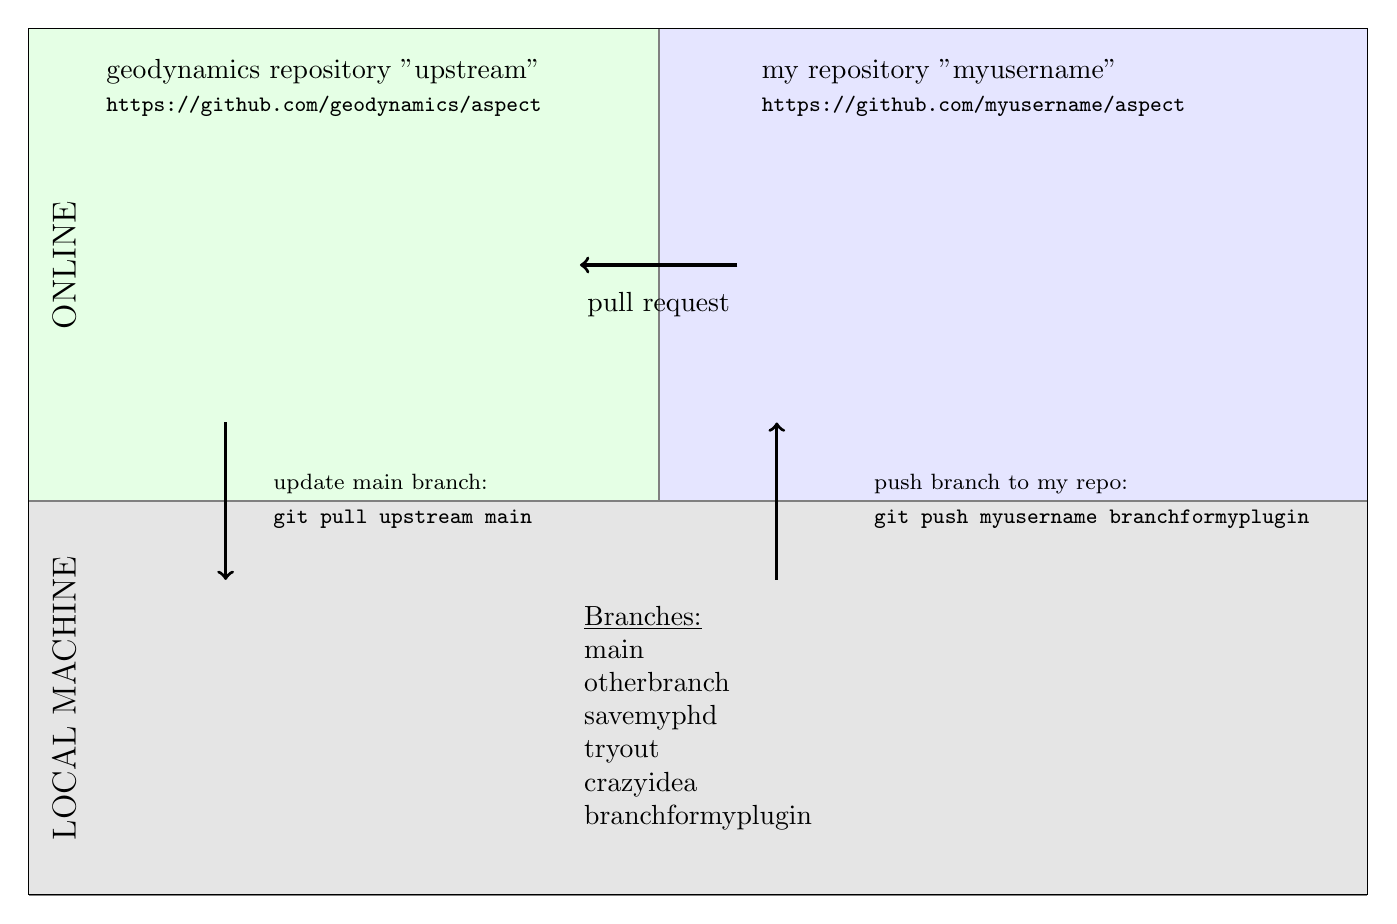
\begin{tikzpicture}
\draw[step=0.5cm,gray,very thin] (0,0) grid (17,11); %background grid

\draw[fill=gray!20] (0,0) rectangle (17,5);
\draw[fill=green!10] (0,5) rectangle (8,11); 
\draw[fill=blue!10] (8,5) rectangle (17,11); 

\draw[gray,thick] (0,5) -- (17,5); %horizontal line
\draw[gray,thick] (8,5) -- (8,11); %vertical line
%\draw[thick] (12,5) -- (12,11); %vertical line

\node[align=left] at (3.75,10.25) {geodynamics repository "upstream"\\ \footnotesize \verb"https://github.com/geodynamics/aspect"};

\node[align=left] at (12,10.25) {my repository "myusername"\\ \footnotesize \verb"https://github.com/myusername/aspect"};

\node[rotate=90] at (0.45,8) {\large ONLINE};
\node[rotate=90] at (0.45,2.5) {\large LOCAL MACHINE};

\draw[->,very thick] (9,8) -- (7,8);
\node[align=left] at (8,7.5) {pull request};

\node[align=left] at (8.5,2.25) {\underline{Branches:}\\main\\otherbranch\\savemyphd\\tryout\\crazyidea\\branchformyplugin};

\draw[->,very thick] (2.5,6) -- (2.5,4);
\node[align=left] at (4.75,5) {\footnotesize update main branch:\\
\footnotesize \verb"git pull upstream main"};

\draw[->,very thick] (9.5,4) -- (9.5,6);
\node[align=left] at (13.5,5) {\footnotesize push branch to my repo:\\
\footnotesize \verb"git push myusername branchformyplugin"};

\end{tikzpicture}


%..............................................
\paragraph{Very concretely, if you wish to contribute:} 

Let us assume that you have found a typo in the file ``physics.cc'' and you wish to 
fix this problem. 

\begin{enumerate}
\item
If this is the very first time you use git, the following instruction is not needed. If not, 
make sure that your terminal points at your main branch:
\verb"$ git checkout main"

\item
Then, make sure you update your local version:
\verb"$ git pull upstream main" 
and also update your own repo online:
\verb"$ git push username main"

\item
Create a new branch with a self explanatory name:
\verb"$ git branch fix_typo"
Then do \verb"$ git branch" to see all your branches. The one that is coloured is 
the active branch. In order to switch to this new branch, do 
\verb"$ git checkout fix_typo". Redo \verb"$ git branch" to verify that 
the branch 'fix\_typo' is highlighted.

\item
Edit the file physics.cc, correct the typo, save and exit. 
Do \verb"$ git status" and you should see the filename highlighted next to 'modified'. 

\item before we go any further, we need to run the indenting script with astyle. 
In the build directory run \verb'$ make indent'.
Note that you need a specific version of astyle, see \url{https://github.com/geodynamics/aspect/wiki/Indenting-code-and-installing-the-correct-version-of-astyle} 

\item add a changelog entry in doc/modules/changes. Look at the entries and find the one that resembles your contribution the most. Use it to 
write your entry.

\item If this is the only modification you wish to communicate, you then need to add and commit 
it as follows:
\begin{verbatim}
$ git add physics.cc
\end{verbatim}
If you do \verb'$ git status' again, the file should have changed colour. 
Then do
\begin{verbatim}
$ git commit -m "message"
\end{verbatim}
where 'message' is a very short description of the modification (e.g. 'I fixed a typo').

\item We now need to bring this modification online 
\begin{verbatim}
$ git push myusername fix_typo
\end{verbatim}

\item You are nearly done. The last step takes place on github.com: when you log onto 
your own github fieldstone page, you should see a large green rectangle "Compare and pull request".
Click on this button, follow the instructions.

\item a new page opens, entitled "Open a pull request" (PR). If necessary, add a detailed description of 
the pull request (this makes sense when you contribute a piece of code, or a whole new section, etc ...).
Later you will be able to review the requested changes at the bottom. In the end, simply click "Create pull request".

\item Once you have done so, \aspect developers will then review it. 
If they have no comment, the PR will be accepted and your modification will 
then be incorporated in the main repo. If they have comments, you will be notified via github and a 
back-and-forth discussion will ensue until the PR is accepted. 

\item if the reviewers have comments. Edit/change your file(s). 
Then add these (\verb'git add ...'), and commit again (\verb'git commit -m "msg"')
and push as before. 



\item After the PR has been accepted, the branch is no longer needed. Switch back to your local main branch:
\$ \verb"git checkout main ".
Update your local main and online repo (see step \# 2) and then delete the no-longer-needed 
branch as follows:
\begin{verbatim}
$ git branch -d fix_typo
\end{verbatim}
\end{enumerate}

-----------------------------------

If there is a pb with your PR and u need to rebase. For example if your 2 PRs modify the same line (say for example reference.bib - 
in that case better spread your changes to different locations in the reference.bib)

\begin{itemize}
\item carry out modifications as required by reviewers
\item \verb'git add' files, and \verb' git commit'
\item \verb'git checkout main'
\item \verb'git branch', make sure you are indeed back on main
\item \verb'git pull upstream main'. depending how much happened in the last hours/days it will display a bunch of files/updates
\item \verb'git checkout my_branch'
\item \verb'git rebase main'. Follow instructions, resolve conflicts in indicated files. 
\verb'git add problematic_file'. 
Finish with \verb'git rebase --continue'. 
\item \verb'git push -f cedrict my_branch'
\end{itemize}

git config --global core.editor "vim"




%%%%%%%%%%%%%%%%%%%%%%%%%%%%%%%%%%%%%%%%%%%%%%%%%%%%%%%%%%%%%%%%%%%%%%%%%%%%%%%%%%%%%%%%%%%%%%%%%
\newpage

\subsection{Contributing a cookbook in \aspect}

\begin{enumerate}
\item Download/update/install \aspect 
\item In the cookbooks folder, create a new folder: \verb'$ mkdir my_cool_setup'
\item In this folder, place your .prm file, say my\_cool\_setup.prm
\item Make sure your .prm file is clean, commented, and contains a header with a concise
description of what the experiment is, and/or in which publication it originates.
\item In the folder, create a new folder:  \verb'$ mkdir doc'
\item In this folder create the file my\_cool\_setup.md file which contains the 
text for the cookbook. Look at other cookbooks md files for examples of how 
to include a figure, an equation, cite publications, etc ...
\item Place in this same folder all figures pertaining 
to the cookbook entry in the manual. 
\item go to \verb'/doc/sphinx/user/cookbooks/' and add your cookbook to the list in 
(for example) \verb'geophysical-setups.md'
\item if you with to cite publications, add them to \verb'/doc/sphinx/references.bib'
\item In order to generate the manual, go to /doc/sphinx and do \verb"$ make html"
\item If there is no error, you should be able to open the file \verb'/doc/sphinx/\_build/html/index.html'
with firefox
\item if the referencing of the figures does not work correctly, simply do 
\verb'make clean' and then make html again.
\item before you make a pull request, make sure you run \verb'make indent'
\end{enumerate}



%%%%%%%%%%%%%%%%%%%%%%%%%%%%%%%%%%%%%%%%%%%%%%%%%%%%%%%%%%%%%%%%%%%%%%%%%%%%%%%%%%%%%%%%%%%%%%%%%
%%%%%%%%%%%%%%%%%%%%%%%%%%%%%%%%%%%%%%%%%%%%%%%%%%%%%%%%%%%%%%%%%%%%%%%%%%%%%%%%%%%%%%%%%%%%%%%%%
%%%%%%%%%%%%%%%%%%%%%%%%%%%%%%%%%%%%%%%%%%%%%%%%%%%%%%%%%%%%%%%%%%%%%%%%%%%%%%%%%%%%%%%%%%%%%%%%%
\newpage
\subsection{Contributing to fieldstone}

\begin{mdframed}[backgroundcolor=red!5]
This appendix was contributed by E. van der Wiel.
\end{mdframed}


\begin{enumerate}
\item make sure that you  have an account on GitHub (say, \verb"https://github.com/myusername") 
and carry out a proper setup on your local computer as follows:\\
\$ \verb'git config --global user.name "firstname lastname" '\\
\$ \verb'git config --global user.email your@email'

\item On github.com, fork the official fieldstone 
repository to your repository:\\
go to \verb"https://github.com/cedrict/fieldstone" 
and click on the 'fork' button on the upper right corner of the screen.
\item On your machine, in a terminal, clone your repository with \\
\$ \verb"git clone git@github.com:myusername/fieldstone.git". This is now your main\footnote{also 'master', although this term should not be used anymore} branch.

\item On your machine, find your security key \footnote{
Note that you can create a public key as follows: 
{\tt https://help.github.com/articles/generating-ssh-keys/}}
 with \$ \verb"less ~/.ssh/id_dsa.pub" and copy this into github.com 
so you can push to your repository. See \url{https://help.github.com/en/articles/connecting-to-github-with-ssh} on how to configure github with ssh support (no more login/password to type -- if you have cloned the repository wish ssh, not html).
Please also check the instructions at \url{https://help.github.com/en/articles/connecting-to-github-with-ssh}.  
 
\item create a remote of your (online) repository\\
\verb"git remote add origin git@github.com:myusername/fieldstone.git"
and in order to avoid potential confusion later on, we shall rename our github repo as follows:\\
\$ \verb"git remote rename origin myusername" 

\item Also create a remote of the official version with\\
\$ \verb"git remote add upstream https://github.com/cedrict/fieldstone"

\end{enumerate}


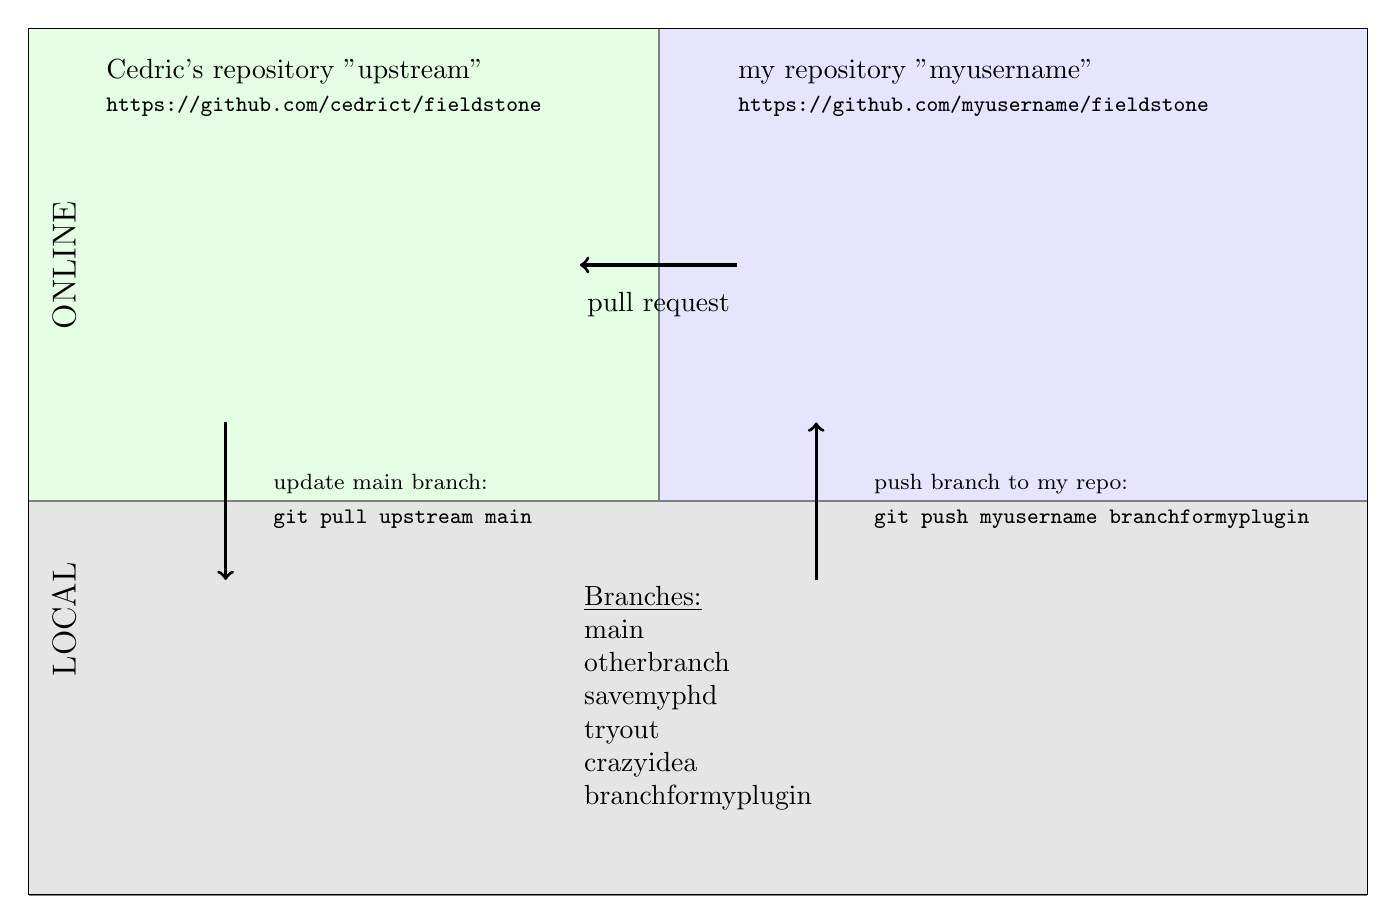
\begin{tikzpicture}
\draw[step=0.5cm,gray,very thin] (0,0) grid (17,11); %background grid

\draw[fill=gray!20] (0,0) rectangle (17,5);
\draw[fill=green!10] (0,5) rectangle (8,11); 
\draw[fill=blue!10] (8,5) rectangle (17,11); 

\draw[gray,thick] (0,5) -- (17,5); %horizontal line
\draw[gray,thick] (8,5) -- (8,11); %vertical line
%\draw[thick] (12,5) -- (12,11); %vertical line

\node[align=left] at (3.75,10.25) {Cedric's repository "upstream"\\ \footnotesize \verb"https://github.com/cedrict/fieldstone"};

\node[align=left] at (12,10.25) {my repository "myusername"\\ \footnotesize \verb"https://github.com/myusername/fieldstone"};

\node[rotate=90] at (0.45,8) {\large ONLINE};
\node[rotate=90] at (0.45,3.5) {\large LOCAL};

\draw[->,very thick] (9,8) -- (7,8);
\node[align=left] at (8,7.5) {pull request};

\node[align=left] at (8.5,2.5) {\underline{Branches:}\\main\\otherbranch\\savemyphd\\tryout\\crazyidea\\branchformyplugin};

\draw[->,very thick] (2.5,6) -- (2.5,4);
\node[align=left] at (4.75,5) {\footnotesize update main branch:\\
\footnotesize \verb"git pull upstream main"};

\draw[->,very thick] (10,4) -- (10,6);
\node[align=left] at (13.5,5) {\footnotesize push branch to my repo:\\
\footnotesize \verb"git push myusername branchformyplugin"};

\end{tikzpicture}


%..............................................
\paragraph{Very concretely, if you wish to contribute:} 

Let us assume that you have found a typo in the file "physics.tex" and you wish to 
report the problem to me. The easiest way is to write me an email with the nature of the 
problem and the proposed fix. Although I will be grateful for your contribution,
this approach can be improved upon by using git's "pull request" command. 



\begin{enumerate}
\item
If this is the very first time you use git, the following instruction is not needed. If not, 
make sure that your terminal points at your main branch:
\verb"$ git checkout master"

\item
Then, make sure you update your local version:
\verb"$ git pull upstream master" 
and also update your own repo online:
\verb"$ git push"

\item
Create a new branch with a self explanatory name:
\verb"$ git branch fix_typo"
Then do \$ \verb"git branch" to see all your branches. The one that is coloured is 
the active branch. In order to switch to this new branch, do 
\verb"$ git checkout fix_typo". Redo \verb"$ git branch" to verify that 
the branch 'fix\_typo' is highlighted.


\item
Edit the file and correct the typo, save and exit. 
Do \verb"$ git status" and you should see the filename highlighted next to 'modified'. 

\item If this is the only modification you wish to communicate, you then need to add and commit 
it as follows:
\begin{verbatim}
$ git add physics.tex
\end{verbatim}
If you do git status again, the file should have changed colour (?). 
Then do
\begin{verbatim}
$ git commit -m "message"
\end{verbatim}
where 'message' is a very short description of the modification (e.g. 'I fixed a typo').

\item We now need to bring this modification online 
\begin{verbatim}
$ git push myusername fix_typo
\end{verbatim}

\item You are nearly done. The last step takes place on github.com: when you log onto 
your own github fieldstone page, you should see a large green rectangle "Compare and pull request".
Click on this button.

\item a new page opens, entitled "Open a pull request". If necessary, add a detailed description of 
the pull request (this makes sense when you contribute a piece of code, or a whole new section, etc ...).
You can review the requested changes at the bottom. In the end, simply click "Create pull request".

\item Once you have done so, I will receive an email which notifies me of the pull request. I will 
then review it. If I have no comment, I will accept the PR and your modification will 
then be incorporated in the master repo. If I have comments, you will be notified via github and a 
back-and-forth discussion will ensue until I accept the PR. 

\item After the PR has been accepted, the branch is no longer needed. Switch back to your local master branch:
\$ \verb"git checkout master ".
Update your local master and online repo (see step \# 2) and then delete the no-longer-needed 
branch as follows:
\begin{verbatim}
$ git branch -d fix_typo
\end{verbatim}
\end{enumerate}

\newpage
\begin{center}
\includegraphics[width=9cm]{images/github/1}\\
\includegraphics[width=9cm]{images/github/2}\\
\includegraphics[width=9cm]{images/github/3}\\
\includegraphics[width=9cm]{images/github/4}\\
\includegraphics[width=9cm]{images/github/6}\\
{\captionfont Screen captures of the procedure described above as 
carried out by E. van der Wiel on his Apple laptop.}
\end{center}
















































\newpage
%%%%%%%%%%%%%%%%%%%%%%%%%%%%%%%%%%%%%%%%%%%%%%%%%%%%%%%%%%%%%%%%%%%%%%%%%%%%%%%%%%%%%%%%%%%%%%%%%%%%%%%%%
In what follows we summarize the most important commands one should and remember while working with github. 
After creating an account one can 'fork' a repository (repo) in the online environment. This repository is a 
copy from the master directory of the developer and should not be used to adapt or change, as changes from the developer (updates) should be obtained in this 'fork', or as it could also be called; your master branch. 
  
In order to be able to work within a repository, for instance, to run and compile different programs, you should have you own branch of the repository in which YOU CAN make changes. The following commands should be used to make, copy and publish your own version of the repo to your local device and the online github environment.

\begin{center}
\begin{tabular}{p{6cm}|p{9cm}}
\textbf{command} &  \textbf{what it does} \\
\hline
  git branch & shows all branches of your repository and highlights the one you're in. \\
  git checkout -b \textless my\_own\_branch\textgreater & This makes your own branch called "my\_own\_branch". \\
  git push origin \textless my\_own\_branch\textgreater & This pushes your own, local, branch to as a second branch in the online repo of github. \\
  git checkout \textless name\textgreater & changing the branch your working in (e.g. master or my\_own\_branch). Or replace the name with a hyphen to switch to the last branch.\\
  git branch -d \textless my\_own\_branch\textgreater & Delete your local branch. \\
  \end{tabular}
\end{center}

  The following commands should be used in order to update your own local branches from updates made by somewhere else (upstream/master is the main repository). One should do this for the local master branch and, where possible as well for the different local branches you have committed changes to already. 

  
\begin{center}
\begin{tabular}{p{6cm}|p{9cm}}
\textbf{command} &  \textbf{what it does} \\
\hline
git checkout master & To make sure you are in the right branch \\
  git fetch upstream & to fetch updates from upstream repositories to you own local branch (e.g. to update your master branch. \\
  git merge upstream/master & Command to update the branch with the fethched repo from 'upstream'. \\
  git push origin master & To level your own online repository again with the one on your local drive (and thus the one upstream). \\
  git checkout \textless my\_own\_branch\textgreater & To switch to your own adapted branch of the repo. \\
  git merge master & Used from another branch working directory to combine the new released version of the master repo with the one where all your own changes are put. -\textgreater Then git finds all conflicts in different files which you need to resolve. \\
  git add . & This adds the resolved issues in your own local branch (not master). After which you are able to commit and push your changes back to the online respository. 
\end{tabular}
\end{center}


While you are working in your own branch you can change, add or delete files in any amount you want. However, always check whether your changes do not inflict the outcome of for instance your code. And when uploading from your terminal: if you commit and then push from master branch your changes will automatically be inserted in the online version of your master branch, when done from another branch it will be shown as a pull request towards your master branch. This request can than, for instance be forwarded to the main repo.\\

\begin{center}
\begin{tabular}{p{6cm}|p{9cm}}
\textbf{command} &  \textbf{what it does} \\
\hline
  git commit -a & This will send your changes/updates from your branch as a commit to your own local branch. \\
  git push origin \textless changes\textgreater & To update the remote repository (on Github) from you local repository (in this case the 'changes' branch). (Actually upload the new version). Online one can then judge what to do with it. !! this is a pull request towards your own fork/local\_branch \\ 
  git status & Showing the status of your current branch; it shows which files are different between the master file and your adapted branch. \\
  git diff \textless changes\textgreater& This shows the exact differences between the different branches; one can simply ask for the difference between two branches when pwd in one branch ask for the other branch. \\ 
  git merge \textless my\_own\_branch\textgreater & When used from the master branch (or any other???) this accepts the changes made in your branch and puts them in your local(!) master branch. \\ 
  git pull origin master & if the main repository changes, one can pull the newest version towards it's own master file. While keeping your own branches alive with you own changes and vica versa: by running this command the origin/master (remote file) will be cloned and updated to the working branch you are in. \\
  git stash (apply) & ?? While updating your local branch, sometimes git wants to overrule your own changes, with this command you can 'stash' them to look at the differences later. ?? \\
\end{tabular}
\end{center}

